% Geometry, font
\documentclass[12pt, letter]{article}
\usepackage[margin=0.8in]{geometry}
\usepackage[T1]{fontenc}
\usepackage{fourier}
\usepackage{titling}
\setlength{\droptitle}{-5em} 
\usepackage[parfill]{parskip}
\usepackage{graphicx}
\graphicspath{{imgs/}}
\usepackage{hyperref}

% Math stuff
\usepackage{amssymb}
\usepackage{amsmath}
\usepackage{bm}

% Code Highlighting
\usepackage{minted}
\usemintedstyle{solarizedlight}

\author{Zach Neveu}
\title{ Day 23 Notes }

\begin{document}
\maketitle
\section{Agenda}%
\label{sec:agenda}
\begin{itemize}
	\item Review of Flow Networks
	\item Solving Max Flow Problsm
	\item Announcement: Grading too slow, expect delays
	\item Announcement: reading, project
\end{itemize}

\section{Max Flow}%
\label{sec:max_flow}
\begin{itemize}
	\item Directed graph
	\item Capacities - can be different in each direction
	\item Single pipe - pos flow one direction means negative flow in other direction
	\item 2 special nodes: source and sink where conservation doesn't apply
	\item Value leaving source is total value of flow
\end{itemize}

\subsection*{Solving Max Flow Problems}
\begin{itemize}
	\item Given nodes $u,v$, the \textbf{residual capacity}, $c_f(u,v)$ is the additional capacity left in the pipe from $u \to v$
	\item Critical Idea: In the residual network, if a path from source to sink exists with all positive residuals, then the flow is not optimum because it can be increased along this path.
	\item above question fair game on quiz\ldots
	\item Given a flow network and a flow, an augmenting path is a simple path (no cycles) from s to t in the residual network. The residual capacity of an augmenting path is the minimum residual capacity of the edges on the path.
	\item \textbf{Ford-Fulkerson Algorithm}:
\begin{minted}{Python}
# Ford Fulkerson Algorithm
def FF(g):
    flow = 0
    while p = is_aug_path(source,sink):
        cfp = residual_capacity(p)
        flow += cfp
\end{minted}
\begin{itemize}
    \item How to prove output is optimal?
\end{itemize}

\section{Ford-Fulkerson Proof}%
\label{sec:ford_fulkerson_proof}
\begin{itemize}
    \item \textbf{Cut}: a cut of a flow network $G(V,E)$ is a partition of $V$ into $S$ and $T=V-S$ such that $s\in S$ and $t\in T$, where s is source, and t is sink.
    \item More simply: If source is at left, Sink is at right, cut the graph with a vertical line.
    \item \textbf{Net Flow} across a cut $(S,T)$ is  $f(S,T)$, the sum of all flow from nodes in S to nodes in T.
    \item \textbf{Note:} Net flow depends on sign, flows going backwards are subtracted.
    \item \textbf{Cut Capacity:} $c(S,T)$ is sum of capacities of all edges from nodes in S to nodes in T.
    \item Cut Capacity is upper bound on net flow across the cut.
    \item \textbf{Minimum Cut}: cut whose capacity is the minimum of all cuts in the network
\end{itemize}

\end{itemize}

\begin{figure}[h]
	\centering
	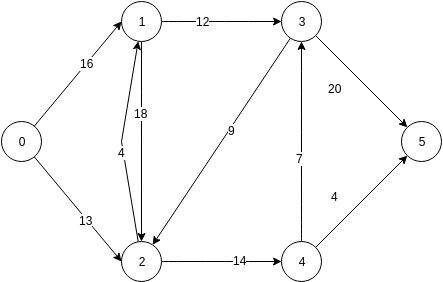
\includegraphics[width=0.8\textwidth]{flow}
	\caption{Max Flow Capacities}
	\label{fig:flow}
\end{figure}

\begin{figure}[h]
	\centering
	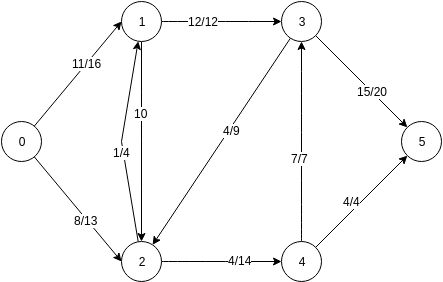
\includegraphics[width=0.8\textwidth]{ex-flow}
	\caption{Example Flow}
	\label{fig:ex-flow}
\end{figure}

\begin{figure}[h]
	\centering
	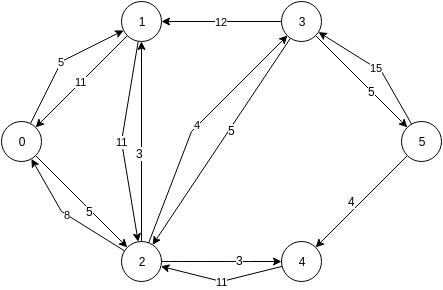
\includegraphics[width=0.8\textwidth]{res-flow}
	\caption{Residual Flow Diagram from Flow in Fig. \ref{fig:ex-flow}}
	\label{fig:res-flow}
\end{figure}




\end{document}
